\documentclass{article}

\usepackage[utf8]{inputenc}
\usepackage[normalem]{ulem}
\usepackage[left=1.25in,right=1.25in,bottom=1.25in]{geometry}
\usepackage{setspace}\doublespacing
\setlength\parindent{0pt}
\setlength{\parskip}{1em}
\setcounter{secnumdepth}{0}
\usepackage{outlines}
\usepackage{graphicx}
\usepackage{caption}
\captionsetup{justification=centering, width=5in}
\graphicspath{ {imgs} }
\usepackage{hyperref}
\usepackage{tabularx}
\usepackage{color,soul}
\usepackage{comment}

\usepackage[
backend=biber,
style=apa,
citestyle=authoryear,
sorting=nyt,
]{biblatex}
\addbibresource{references.bib}

\title{Astana, a post-socialist city between East and West}
\author{Carla Hyenne}
\date{}

\begin{document}

\maketitle 

\begin{center}
\textit{Literal research question: To what extent are imperial and colonial relations relevant for understanding the contemporary structure (economic and/or social and/or cultural) of your city?}

\textit{Word count including abstract, excuding bibliography: 3811}

\end{center}

\section{Abstract}

Post-socialism characterises ex-Soviet cities after their independence from the Soviet Union.
Astana, the capital of Kazakhstan, was created by authoritarian president Nazarbayev in direct response to Kazakhstan's independence. At the same time, the country was undergoing projects of nation- and state-building, and of economic recovery. As such, Astana was never a city under socialism but still exhibits features of post-socialist cities. In this paper, I use post-socialist theory and take an empirical approach to understand to what extent Astana's contemporary socio-economic structure can be explained by post-socialism. 
I focus on the marketisation of the economy and the stratification of society. 
More than thirty years after Soviet independence, it becomes apparent that cities like Astana warrant a new theory. 
Are mainstream, neoliberal theories useful? Using global cities rhetoric, I will discuss Astana's socio-economic and political position between Europe and Russia in a globalising world, and whether conventional urban theories are sufficient. 
The conclusion is that neoliberal globalisation does not fully explain Astana today. The government's political and economic ambitions for the country are to be understood as an amalgam of ideologies from the east and the west, for which a new categorisation is required.

\pagebreak

The dissolution of the Soviet Union in 1991 left in its wake an enormous project for the ex-Soviet states in East Central Europe (CEE) and Central Asia. The processes of nation building, state building, and economic reform that ensued defined the countries we know today. It is particularly interesting to analyse Astana in the context of post-socialism, because of the way it came to be Kazakhstan's capital. 
Until 1994, the capital was Almaty, but it made strategic sense to move the capital to a north-central location. 

The first reason is Almaty's proximity to the Chinese border, which posed a risk of invasion. It is also surrounded by mountains, making it hard to physically expand and accommodate a larger population. 
Second, Almaty is a well established city, carrying cultural and architectural traditions. This clashed with the intentions of Nursultan Nazarbayev, the first, authoritarian president in power from 1991 to 2018, to build a modern, independent and prosperous image of Kazakhstan. 
Third, the north of the country was predominantly Russian. Situating the capital in the north allowed the State to encourage Kazakh migration northward and promote ethnic integrity.
 Lastly, the president was looking for a tabula rasa to conduct his post-socialist project. Akmola, an industrial city with 200,000 habitants, in a north central location, with better connections to major Kazakh cities, surrounded by steppe, and on the Ishim river, was chosen as the ideal place.

Thus, Astana is a capital city built in direct response to Kazakhstan's independence from the Soviet Union. This is why the question “to what extent is Astana's contemporary socio-economic structure influenced by post-socialism”, is relevant. It will be approached in two parts. First using post-socialist theory, and second using the opposite of socialism - capitalism - to capture how far the city has come from the former.

I will first provide contextual background on Astana since its formation in 1994. Then, I will give a brief review of post-socialist theory, and explain why conventional urban knowledge may not apply to cities like Astana. 
I will focus on two socio-economic features of post-socialist cities to analyse Astana: the marketisation of the economy and the stratifying social structure.
This will lead me to discuss whether post-socialism is still relevant. I will conclude that Astana's contemporary socioeconomy exhibits characteristics of post-socialism, but does not fit as neatly into this category as it may once have. 
However, `conventional' western theories such as the global cities paradigm do not apply to Astana, either. 
Finally I will argue that the social, economic and political landscapes of Astana merit a new analysis, which exists perhaps between socialism and neoliberal capitalism.

\section{Creating a Capital City after Socialism}

The rebuilding of Kazakhstan after independence in 1991 was heavily influenced by president Nazarbayev. The collapse of the USSR offered a great opportunity for politicians in the communist party to become leaders of their independent nations. This resulted in the rise of authoritarian regimes in Central Asia, whereby leaders exercised their power similarly to that of communist leaders of the 20th century. Nazarbayev was accepted thanks to his success in meeting the nation's demands \parencite{isaacs2010papa}. Indeed, the economic prosperity and the emergence of a new middle class with disposable income helped legitimise his regime  domestically and internationally, even if prosperity was not uniform across the country. Nazarbayev stood by his motto ``economy first, then politics'', believing that only with a high standard of living would a country be stable enough for democracy \parencite{kassymbekov_2020}.

Central to Kazakhstan's post-socialist success was the creation of the new capital, Astana. As a tabula rasa for Nazarbayev's ``pet project'' \parencite{koch2010monumental}, it was branded as the image of a modern, prosperous and independent Kazakhstan. It projected the future of the country's society, politics, and economy. Today, the relocation of the capital is seen as one of the most important events that cemented the post-socialist economic and political reforms \parencite{kassymbekov_2020}.

The left bank of the Ishim river is where the new administrative, monumental and recreational buildings are located. 
They were developed on mostly virgin land since Akmola existed predominantly on the right bank. 
In this sense, the urban landscape changed dramatically and quickly, which is unusual for a city. The built environment is normally slow to change, in comparison to political and economic structures which can revolutionise in days \parencite{stanilov2007post}. The built environment played an important role in cities after socialism, especially because it was instrumental as a site for political representation under communism. In the case of Astana, the urban landscape not only changed in parallel with, but created a new society and economy. 

\begin{figure}[h!]
	\centering
	\captionsetup{labelformat=empty}
	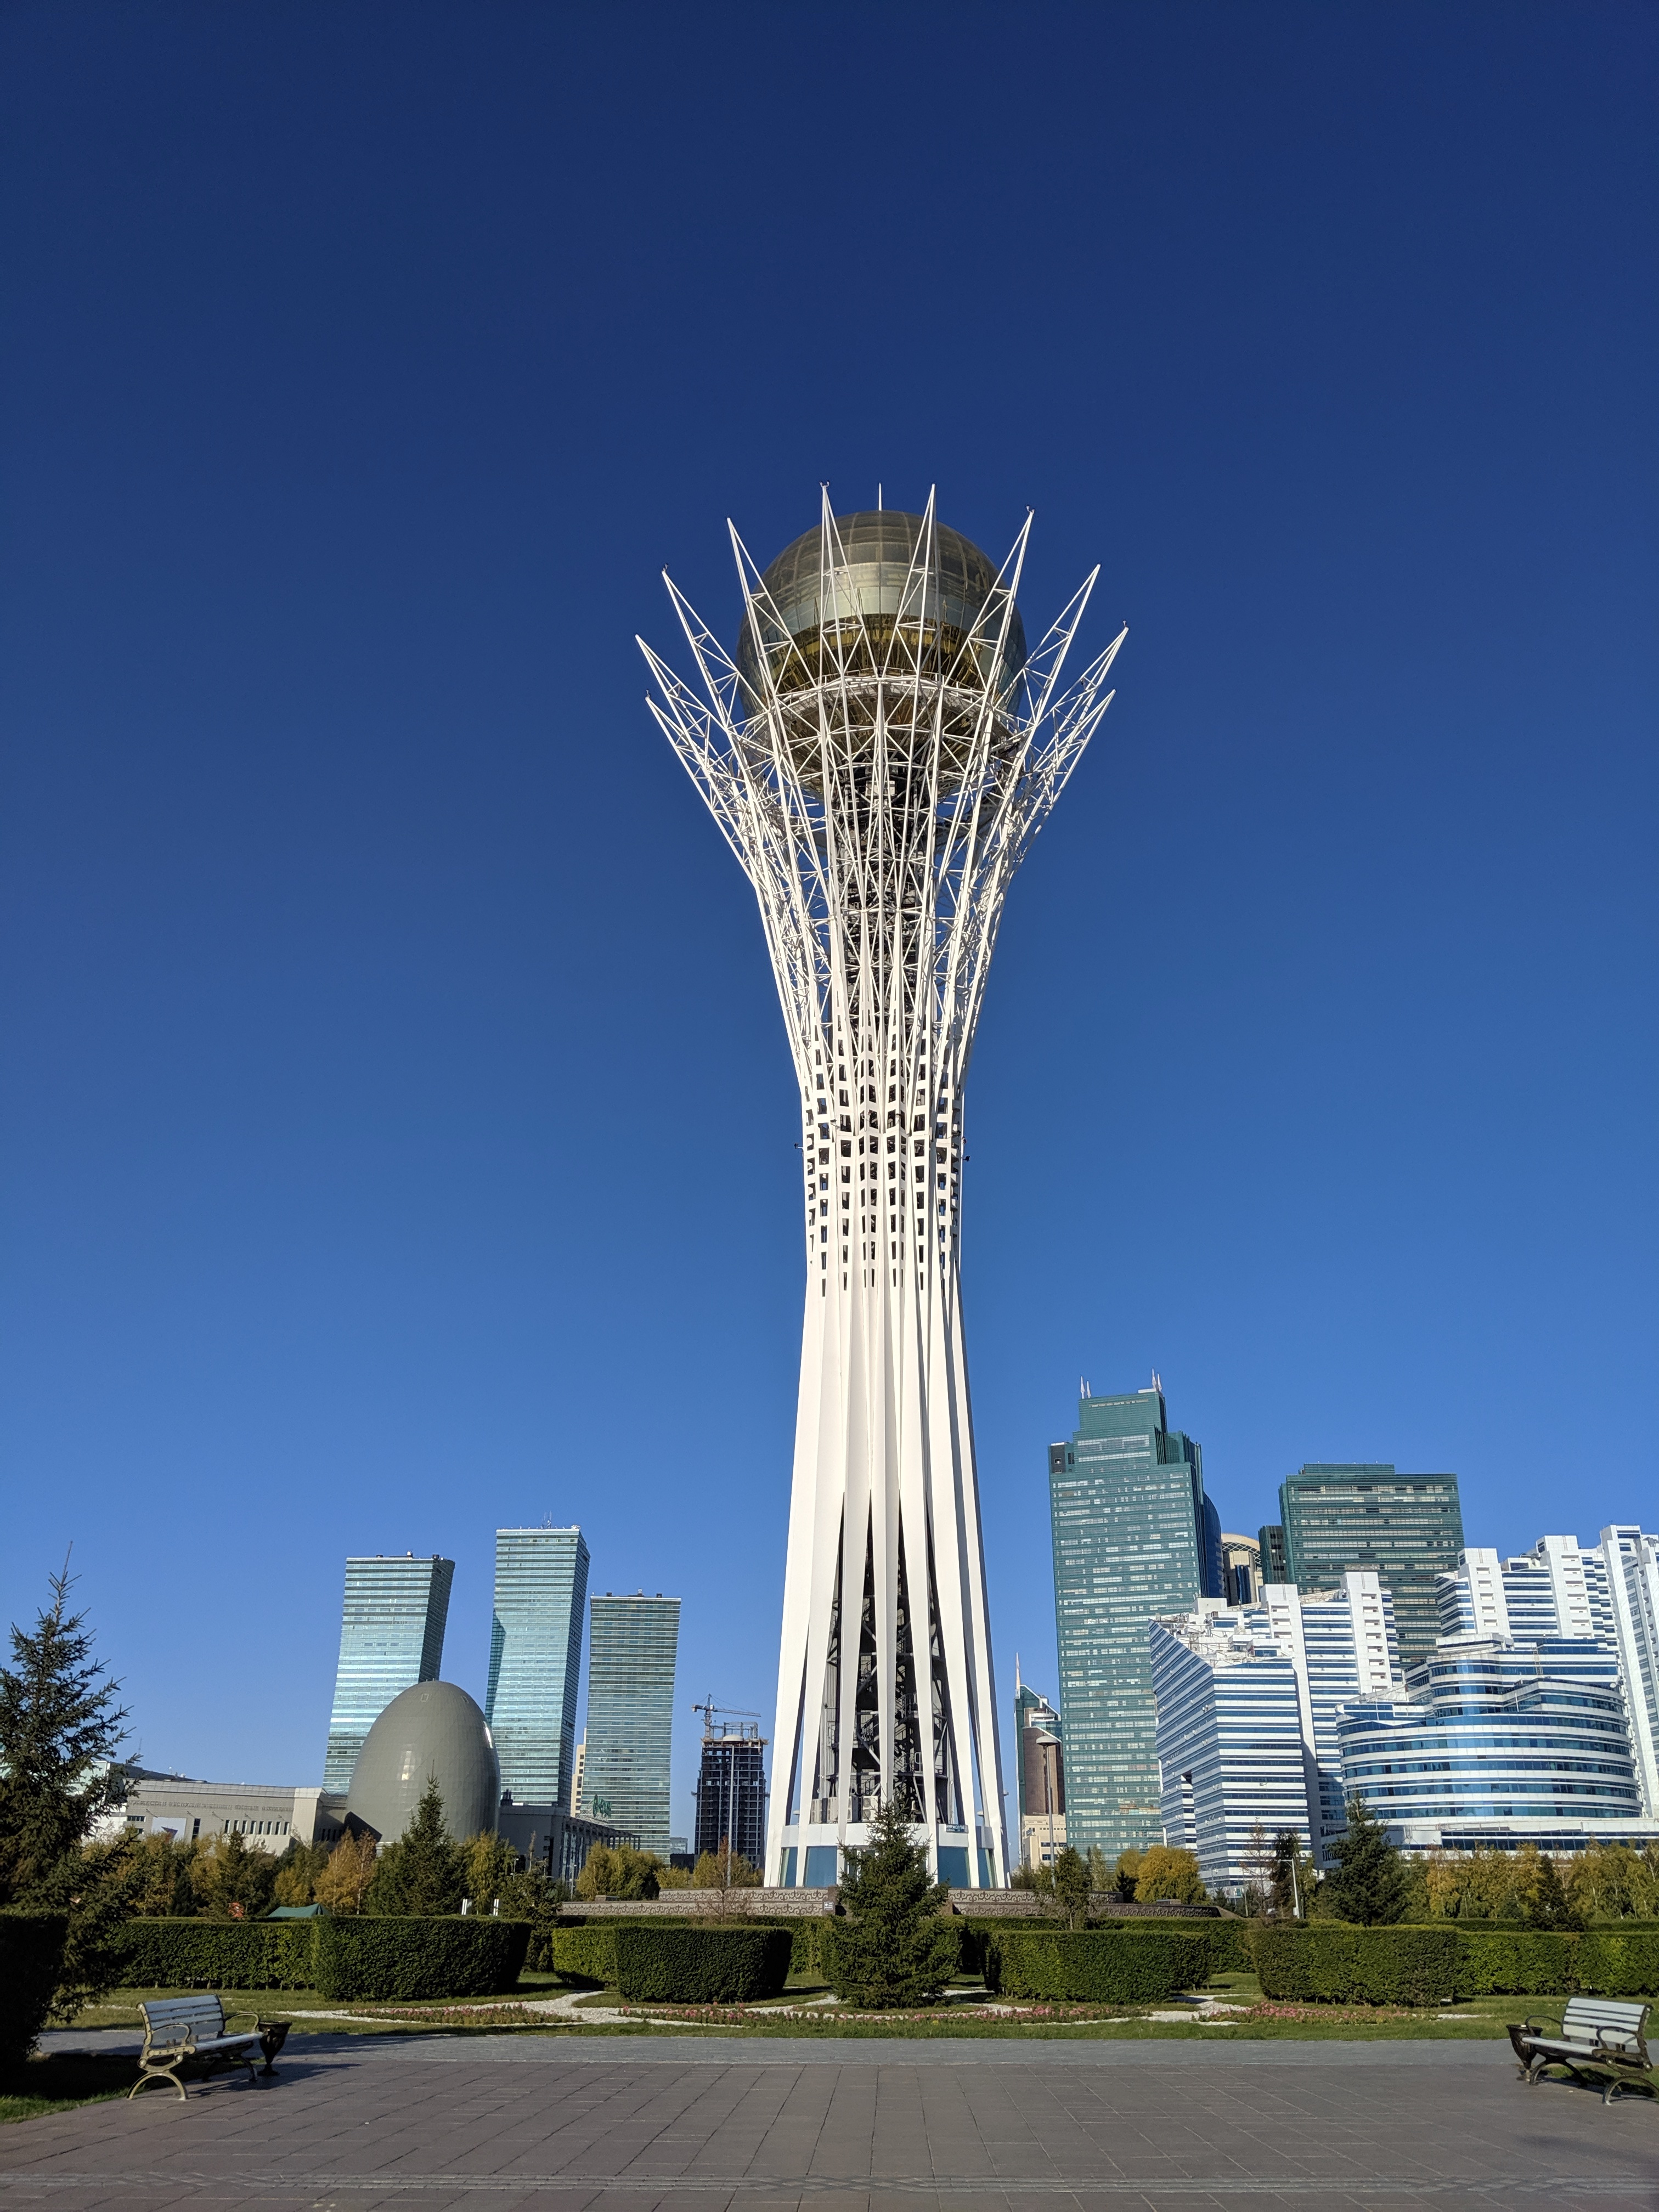
\includegraphics[width=0.45\textwidth]{astana_modernity}
	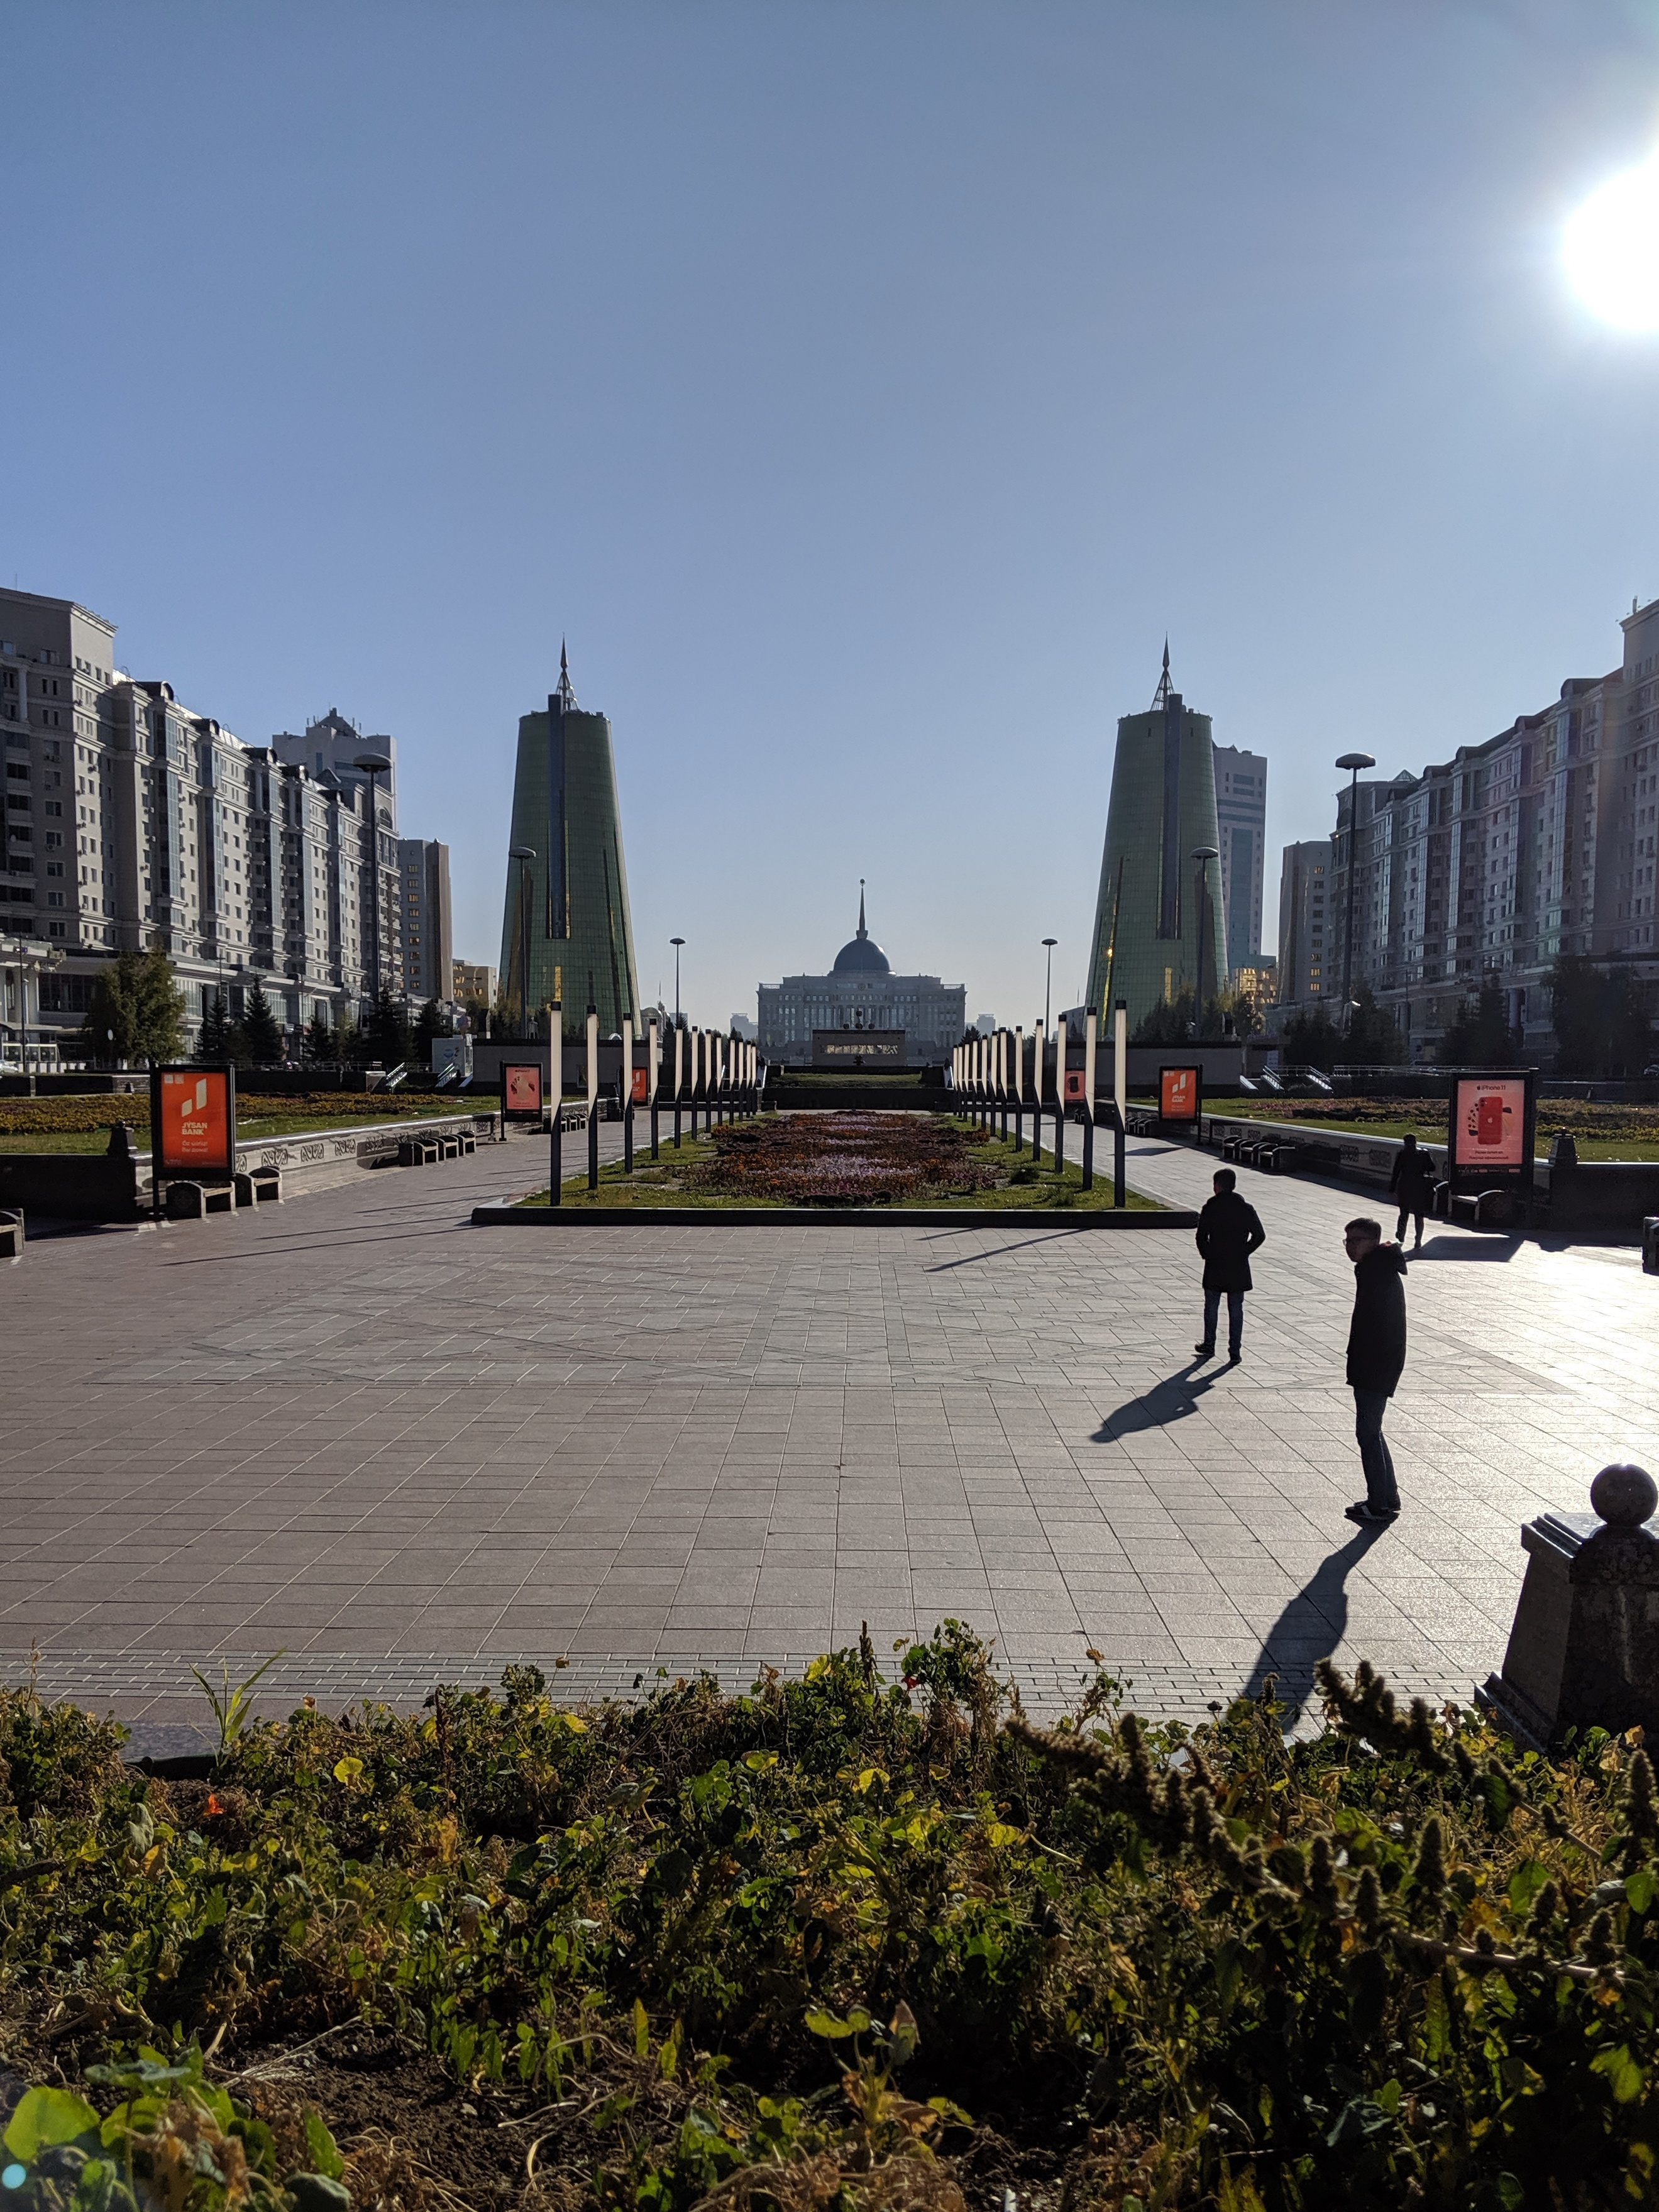
\includegraphics[width=0.45\textwidth]{astana_modernity15}
	\caption{Left: Baiterek tower on Nurzhol Bouldevard, a pedestrian walkway cutting through the administrative and business districts. The tower is a symbol of post-independence and the pinnacle of modernity in Astana's built environment.
	\\Right: also on the Nurzhol Boulevard, the presidential palace lined by two golden towers housing government offices.}
\end{figure}

There was a strong segregation between Russians and Kazakhs during socialism. The nation-building emphasised the importance of social integrity, and displayed the country's multi-ethnic and multi-religious composition as a strength. The government had to create opportunities for the populations to mix while promoting Kazakh culture. It was important that the Russian community not dominate the capital, so that Kazakhstan could be seen as a self-standing nation, not controlled by or relying on the imperial power. 
Astana became the place to promote (modern) Kazakh culture. 
Campaigns launched to attract Kazakhs to the capital, Kazakh language was promoted in schools, and recently, Kazakh proficiency became mandatory for government officials. Efforts were successful: between 1991 and 2019, the Kazakh population of Astana surged from 44\% to 78.2\% \parencite{unfpa2020wekazakhstan}, a significant majority. 
Internal migration is the primary driver of the population growth. As a self-made man himself, Nazarbayev served as an inspiration to move to Astana for a new life. He came from a poor family in a rural town, worked on a steel mill, and paved a way for himself in politics by using his working class background and intellect. All over Kazakhstan, people are attracted by the job opportunities and the promise of a better life that Nazarbayev successfully portrayed.

Given its history, Astana proves interesting to study as a post-socialist city precisely because it did not exist under socialism, but was built from the ground up as a post-socialist achievement.

\section{Why are post-socialist theories relevant?}

From the 1990s analyses of ex-Soviet cities emerged to explain the transition from a socialist system towards a new socio-economic system (\cite{smith1996socialist}, \cite{sailer1999characteristics}, \cite{hirt2013whatever}). The challenge for ex-Soviet countries in CEE and Central Asia was to rebuild the nation, the state, and the economy; they focused on processes of democratisation and marketisation \parencite{ferenvcuhova2016introduction}. 
Conventional urban theories like the political economy perspective, the global cities paradigm, or neo-Weberianism \parencite{haussermann2005european} are not sufficient to explain cities in this context.

For one, they don't account for the nation and state building projects, two major processes that shaped the socio-economic and spatial structures of post-socialist cities.
Second, the political economies of (post) socialist and capitalist states are different, and the laws of capital that explain cities in Western Europe do not translate \parencite{hirt2013whatever}. Plus, economic forces were not the only determinants of post-socialism. In Astana, Nazarbayev's presidency played a critical role.
Third, although Astana has an increasing number of transnational headquarters, financial institutions and producer services, it is not a global city and, as we will discuss later, it is not aspiring to be one.
Lastly, neo-Weberianism describes the government meeting the demands of the population through public land ownership, welfare policies and citizen participation \parencite{haussermann2005european}. This is not the case in Kazakhstan. The primary task was to rebuild the economy, which created a middle class but also engendered inequalities, which were not countered by the welfare state.

Urban knowledge needs to be situated in a time and place, and western theories cannot be exported as-is to a post-socialist, Central Asian city like Astana. This critiques the `universality' of urban theories, that are realistically only applicable to the global North (\cite{ferenvcuhova2016accounts}, \cite{robinson2013ordinary}), and characterises cities on the periphery of the neoliberal world system as backwards and needing to catch up to western ideals.
% This distinction is visible in global North cities who dominate the world's finance and trade.

Therefore, post-socialist theories are necessary to understand processes that states underwent after communism. The analysis is conducted from one of two perspectives: by comparing the city to the socialist ideal \parencite{sailer1999characteristics}, or by following `conventional' literature and comparing to the capitalist city (\cite{smith1996socialist}, \cite{haussermann1996socialist}). Although the perspectives differ, outcomes are similar. Using the second approach, Smith summarises the differences between (post) socialist and capitalist cities by their ``general physical organisation, socio-economic differentiation and ethnic segregation'' \parencite{smith1996socialist}. Using the first approach, Sailer-Fliege develops a comparative model of socialist and post-socialist city ideologies in CEE that overlap with Smith. Even though Sailer-Fliege developed the model specifically for CEE cities, the overarching themes are still applicable to Central Asian cities like Astana.

To analyse the extent of post-socialism in Astana's contemporary socio-economic structure, I will use two post-socialist ideologies. 
First, the marketisation of the economy. This is the transition from a centrally planned economy with priority given to `productive' economic sectors, towards a market economy and the take off of the tertiary sector. 
Second, the transition from an egalitarian society towards a stratified society, with rising social inequalities and growing differences in living conditions.

Afterwards, I will discuss the extent to which post-socialism is useful to understand Astana today, and whether it can be better explained with a capitalist perspective. It makes sense for post-socialist urban theories to exist, but should not be the end-all theory for ex-Soviet cities; especially because it is process of transition, to a state somewhere between socialism and capitalism.

\section{Post-socialism in Astana's socio-economic structure}

\subsection{Neoliberalisation of the economy}

The collapse of the Soviet Union created an economic crisis in Kazakhstan. The country had to pivot from a centrally planned, industrial economy trading with the Soviet Bloc, to a marketised economy opening up to the world. Today, the economy of the Akmola region where Astana is located is predominantly based on industry, agriculture and manufacturing (over 50\% of the GRP since 2010). In contrast, Astana's economy is predominantly based on wholesale and retail trade, real estate activity, and professional scientific and technical activities (over 40\% of its GRP since 2010)\footnote{Calculation based on the sum of the average GRP of the three most lucrative economic sectors (agriculture, industry, manufacturing for Akmola, and wholesale and retail trade, real estate and processional scientific and technical activities for Astana) divided by the average total GRP between 2010-2020}. In parallel, employment is highest in wholesale and retail trade, followed by construction and education. Though construction is the fourth largest contributor to Astana's GRP, the disparity between the most lucrative and most employable sectors is visible: the construction and education sectors pay relatively less than trade and real estate.

Astana is in line with the post-socialist transition towards a de-industrialised economy with a growing tertiary sector. To marketise and globalise the economy after socialism, the government took a Eurasian approach and looked for opportunities outside the Soviet Bloc, in Europe and Asia. For example, Astana has the Astana International Financial Centre (AFAIC) whose aim is to ``position itself as a global centre for business and finance'' \parencite{aifc}. Astana was deliberately chosen as the location for new economic sectors and investments in technology, innovation and entrepreneurship as Kazakhstan diversified its economy. Special economic zones were created to attract foreign investors and businesses, especially in the technology industry, and the number of small and medium enterprises grew fourfold between 2005 and 2020.

\subsection{Commodification of housing}

Another feature of Astana's post-socialist economy is the real estate market. It emerged when housing changed from a social service to a commodity, and resulted in a significant decrease of public investments in housing and an increase in prices. 
By reducing its role in the provision of housing, the government created conditions for private investors and individuals to build and own homes. The beginning of the 1990s had a significant drop in housing construction compared to Soviet times. But, the neoliberalisation of the housing sector, with the introduction of bank loans and mortgages led to a rapid increase in construction in the mid 2000s \parencite{unece2018housing}.

Today, the biggest participants in Kazakhstan's housing market are the real estate developers \parencite{unece2018housing}. According to national statistics, between 2005 and 2018, the volume of services related to real estate in Astana grew from 29.8 to 267.5 million tenge.
At the same time, the cost of housing tripled between 2001 and 2015 \parencite{seitz2021urbanization} and it has become unfeasible for most households to move to the city despite the job opportunities and higher wages. To put it into perspective, Astana is 240\% more expensive to live in than the national average \parencite{seitz2021urbanization}. The housing affordability crisis is further exacerbated by the virtual inexistence of the rental market: in 2015, over 80\% of the dwellings in Astana were owner-occupied \parencite{seitz2021urbanization}.

Commodification hasn't meant a complete abandonment of housing by the government. Launched in 2016, the Nurly Zher programme aims to facilitate housing construction, provide access to mortgages, and access to housing for vulnerable populations. However, this includes military and government staff, but does not cover the low-middle class who isn't eligible for the extremely limited social housing \parencite{unece2018housing}.

\subsection{Social inequalities}

The neoliberalisation of the economy and of the welfare state contributed to the socio-economic inequalities in Astana, a trend visible across post-socialist cities. A middle class emerged, but the welfare state did not support disadvantaged populations who moved in. The surge in housing prices can be explained by projections that grossly underestimated the population growth. Today, Astana has more than 1 million inhabitants, and was originally projected to have 600,000 by 2030 \parencite{masterplan2001}. Contrary to post-socialist trends, Astana did not experience an urban-to-rural migration observed of CEE cities due to growing unaffordability. Instead, the promise of employment and a better life attracted rural Kazakhs to the new capital. But not everyone benefited equally from the new economic structure.

The influx of construction labour created pressure in the city, and reinforced sociospatial inequalities especially with the highly educated population with high-skilled jobs.
Despite the government's promotion of ethnic mix in the 1990s, the rural Kazakh population who migrated to Astana for work lives in the city but with a strong ``rural mentality'' that is not cosmopolitan \parencite{koch2014bordering}. They have a lower income, live in the right bank and in the remaining Soviet era housing complexes that escaped demolition but are sometimes in need of reconstruction.

On the other side of the river are glamorous shopping malls like Khan Shatyr, luxurious residential condos, and impressive government buildings like the Presidential Palace. The modern and consumerist amenities were built to cater to the emerging middle class. To the extreme, marketisation created a capitalist oligarchy whereby the Kazakh elites\footnote{The Kazakh elites are for the most part people in government, or related to the people in government and especially to Nazarbayev} living in Astana profit disproportionately from the wealth created by the oil and gas industries in the rest of the country \parencite{gallo2021three}.

Nonetheless, Astana's economic success since independence has improved the standards of living and created a more equal society. The poverty gap has been closing over the last decades. Educational attainment is high, and students come from all over the country to attend Nazarbayev University that opened in 2010. The inequality index has been comparable to north European countries in the last few years. % Gentrification is limited in Astana, but this has to do with its recency more than because of social interventions \parencite{required}

\section{Astana after post-socialism - a melting pot of east and west?}

% In conclusion, socio-economic inequalities rose in Astana after socialism and were spatially patterned on either side of the Ishim. The soaring housing prices, the contrast between the large but low-paying construction sector and the lucrative real estate and wholesale and retail trade industries, and the \sout{neoliberalisation of the welfare state} are all characteristic of post-socialism. However the inequalities aren't as pronounced today as they were under socialism.

It has been thirty years since the dissolution of the Soviet Union, an era that spanned fifty-five years in the history of a nation that is thousands of years old. Post-socialism is a transitional process characterised by rapid change, and, by definition, assumes there exists a state after which the cities are no longer `post-socialist' per se. 
As we have seen, Astana's economy and society was definitely shaped by post-socialism, even if social inequalities are not as pronounced as under socialism. But, to understand the degree of influence of post-socialism on Astana's socio-economic structure, we should ask: marketisation, globalisation, neoliberalisation, to what extent?

It follows that post-socialism will be phased out. The term is not future oriented. Eventually, all cities will have completed the transition out of Sovietism (if not already), and the outcome of these transitions will look different across all cities. Post-socialist cities will no longer fit into one single category \parencite{hirt2016conceptual}.

What does this \textit{post}-post-socialist city look like? 
There will not be one theory to categorise all post-socialist cities, but if capitalism is the antipode of socialism and the communist regime, it can be used as a benchmark to explain how far cities have come from socialism. However, it cannot fully explain a city like Astana. To illustrate this, I will borrow from one popular urban theory, global cities.

On the surface, Astana looks like an aspiring global city, integrating into the globalised, capitalist economic and financial network, and positioning itself strategically on a global scale. The city is becoming an autonomous force in Kazakhstan and abroad.
But if neoliberalism were the goal for Astana, it would be more obvious in its economy, politics and society. There are multiple reasons why it isn't.

Firstly, Astana is a city on the periphery of the neoliberal `core', geographically, economically and symbolically.  
Geographically, the potential for Astana to reach countries outside Central Asia and Russia is limited, even if it is the most connected city in Kazakhstan by air and land.
Economically, Astana does not have the same resources as other global cities like Dubai. Up to now, Kazakhstan has profited from its wealth of oil and gas but is vulnerable to falling commodity prices \parencite{batsaikhan2017central}. Natural resources attract the majority of foreign investments into Kazakhstan, but this industry is non-existent in Astana. And, it cannot compete in terms of innovation and technology, at least for now.
This is important because what matters in the global economic network is less the geographical connection, but the exchange of knowledge, ideas and capital. Astana's global potential in this sector today is limited.
Symbolically, Astana is closer to Russia than the West. Its regime, culture and population has significant Russian influence. For example, the restriction and censorship of the internet, or local blackouts during protests and elections are reminiscent of recent Russian practices \parencite{freedomhouse2021}.

Moreover, the political landscape is not democratised like in most of the global North. Nazarbayev ruled as an authoritarian leader, elections are not free by Western standards, Nazarbayev's cult of personality is visible all over Astana, and there is considerable corruption in the government. This is not to say that a city must be democratic to be a global city, but that the government's aspirations for Astana are not easily explained with neoliberal and globalisation discourses. Rather, the government promotes nationalist tendencies and rejects the interference of the West in politics and the economy \parencite{koch2013not}. 

Continuing on the political, the economic motivations of the government and the elites are vastly different than that of neoliberal states. Whereas neoliberal governments facilitate capitalism through laws and regulations, to facilitate wealth accumulation of private companies so they may bring prosperity to the city, the Kazakh government's participation in the neoliberal world economy is motivated by the advantages it can bring to its elites \parencite{gallo2021three}. The State is indirectly influencing the economy, especially through dubious contracts and companies that focus on the profitable mining and industry sectors, which do not contribute to the export of knowledge and information.

Thus, it is clear that Astana is not driven by the same ideologies as global cities are. Astana, and Kazakhstan as a whole, are a melting pot of east and west, reflecting their history and landlocked position between Europe, Russia and China, three global superpowers with vastly different socio-politico-economic landscapes. Post-socialism alone cannot explain this unique position, but neither can neoliberal, western theories. The appropriate theory is likely an amalgam of ideologies from the east and west, distinct to Central Asia.

\section{Conclusion}

In conclusion, Astana is undeniably a post-socialist city. Imagined and built from the ground up following Kazakhstan's independence, Astana exhibits many characteristics familiar to post-socialist cities. These include the marketisation of its economy visible by the growth of the tertiary sector, the increase in foreign direct investments, and the commodification of housing; and the rise of socio-economic inequalities due to the economic restructuring and political corruption.

At times, it seems odd to apply post-socialist theory to a city that never existed under socialism per se. Plus, what is taking place can no longer be explained purely with post-socialism; we must look beyond this transitional phase.
To understand Astana's socio-economic trajectory, I applied the global cities paradigm, one of the most popular urban theories since the 1990s. I concluded that Astana's political-economic landscape did not make it an aspiring global city.
 Astana requires a localised theory, which takes into account the socialist past of Kazakhstan and its political uniqueness, to understand its position in a globalising world.


In the end, post-socialist urban theory can help to understand forces that shaped Astana since the 1990s, even if the city begs for a new analysis.
And perhaps, without a Soviet past, Astana would still be called Astana, and not Nur-Sultan - even if the name still lingers, either out of habit or resistance.

%%%%%%%%%%%%%%%%%%%%%%%%%%%%%%%%%%%%%%%%%%%%%%%%%%%%%%%%%%%%%%%%%
%																					OUT TAKES
%%%%%%%%%%%%%%%%%%%%%%%%%%%%%%%%%%%%%%%%%%%%%%%%%%%%%%%%%%%%%%%%%

\begin{comment}
\hfill
\bgroup
\def\arraystretch{1.5}
\begin{table}[h!]
\centering
\begin{tabularx}{\textwidth} {
  | >{\centering\arraybackslash}X 
  | >{\centering\arraybackslash}X |}
	\hline
	\textbf{Smith} & \textbf{Sailer-Fliege} \\ 
	\hline
	General physical organisation & 
	Compact city with slightly less homogeneity; Extensive industrial blight; new industrial areas of urban fringes \\ 
	\hline
	socio-economic differentiation & 
	Deindustrialisation; take-off of the tertiary sector; increase of foreign direct investment; commodification of the housing sector \\ 
	\hline
	Ethnic segregation & 
	Stratified society according to efficiency; sharp rise in social inequalities; suburbanisation; luxurious housing enclaves \\
	\hline
\end{tabularx}
\caption{Post-socialist city characteristics according to two analyses coming from two different angles. Smith, from a capitalist city perspective, and Sailer-Fliege, from the socialist city perspective. The list is not exhaustive.}
\label{table:smith_vs_sailer}
\end{table}
\egroup
\hfill
\end{comment}

\pagebreak

\printbibliography

\end{document}


